\documentclass{article}

\usepackage{spconf,amsmath,graphicx,hyperref}
\usepackage{booktabs,url}
\hypersetup{hidelinks}

\graphicspath{{figures/}}
\newcommand{\cw}{\ensuremath{C-W}}
\newcommand{\wg}{\ensuremath{W-G}}
\newcommand{\crr}{\ensuremath{C-R}}
\newcommand{\dauc}{\ensuremath{\Delta\mathrm{AUROC}}}
\newcommand{\dmrr}{\ensuremath{\Delta\mathrm{MRR}}}

\title{PAIRING-CONTROLLED AUDITING OF CLINICAL AUDIO--METADATA ALIGNMENT:\\
SEPARATING PARTICIPANT CORRESPONDENCE FROM DISEASE TRANSFER}

% ICASSP 2027 is not double blind. Replace both placeholders before submission.
\name{Author names to be inserted before submission}
\address{Affiliations to be inserted before submission}

\begin{document}
\ninept
\maketitle

\begin{abstract}
Clinical audio models increasingly align recordings with patient metadata, implicitly
treating successful correspondence as improved disease representation. Yet metadata mixes
symptoms with demographic and cohort information. We introduce a Pairing-Controlled
Transfer Audit comparing correct pairs, metadata shuffled within disease labels, and
globally shuffled metadata. This separates exact participant-profile correspondence from
label-conditioned association. In UKCOVID, correct pairing improved profile retrieval for
AST-6L and OPERA-CT and strongly retained sex information (matched probe \dauc{} $+0.191$
and $+0.112$), while COVID gains were small and uncertain ($+0.006$ and $-0.002$).
Across UKCOVID and secondary analyses on CODA TB, Cambridge COVID-19 Sounds, and Coswara,
10/11 retrieval and 11/11 sex-probe intervals excluded zero, but 0/11 matched disease
intervals did. Correct alignment also failed to consistently outperform raw audio.
Clinical audio--metadata studies should therefore evaluate correspondence, retained
information, and disease transfer separately.
\end{abstract}

\begin{keywords}
clinical audio, contrastive learning, metadata, confounding, domain shift
\end{keywords}

\section{Introduction}
\label{sec:intro}

Respiratory audio models increasingly combine cough, breathing, or lung sounds with age,
sex, symptoms, smoking status, and medical history. General-purpose audio representations
such as AST, OPERA, and HeAR support this direction
\cite{gong2021ast,zhang2024opera,baur2024hear}. Recent systems go beyond prediction-time
fusion and explicitly align each recording with clinical text derived from the same
participant. RespiraMFM, for example, freezes audio and text encoders and learns an
audio-side projector before downstream multimodal prediction
\cite{siam2026respiramfm}.

The premise is appealing: better audio--metadata correspondence should produce a more
clinically useful representation. It is not guaranteed. Clinical metadata mixes
disease-associated symptoms with demographic background, medical history, missingness,
and variables correlated with recruitment. A contrastive loss cannot distinguish portable
disease evidence from these alternatives; it rewards any feature that identifies the
assigned positive pair. Consequently, improved alignment loss, retrieval, or source-cohort
AUROC may reflect (i) exact participant-profile correspondence, (ii) label-conditioned
population association, or (iii) transferable disease evidence.

We introduce a \emph{Pairing-Controlled Transfer Audit} to separate these claims. Three
otherwise identical projectors receive correct metadata, metadata from another participant
with the same disease label, or globally shuffled metadata. Duplicate-aware retrieval first
checks whether exact pairing was learned; probes then identify retained information; and
covariate-balanced targets test whether that information improves disease prediction. Raw
audio, nonlinear readouts, and calibration transport address alternative explanations.

Our contributions are: (1) a pairing intervention that separates exact profile
correspondence from label-conditioned association; (2) an audit sequence linking
retrieval, information probes, raw references, and matched transfer; and (3) a
multi-dataset, multi-backbone study showing reproducible profile correspondence---most
consistently for sex---without a robust gain in covariate-balanced disease prediction.
Our claim is not that metadata alignment is universally ineffective. Rather, correspondence
learning and disease transfer are distinct empirical claims.

\begin{figure*}[t]
  \centering
  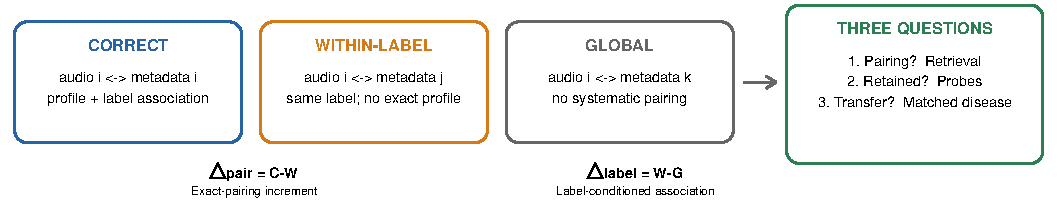
\includegraphics[width=0.98\textwidth]{pairing_audit.pdf}
  \caption{Pairing-controlled audit. Correct and Within-label preserve the same
  label-conditioned metadata distribution in expectation, but only Correct preserves exact
  participant-profile pairing. Retrieval, probes, and matched disease evaluation answer
  three separate questions.}
  \label{fig:audit}
\end{figure*}

\section{Data and Methods}
\label{sec:method}

\subsection{Datasets and evidence hierarchy}

UKCOVID is the discovery dataset \cite{budd2024ukcovid}. After objective audio filtering,
its Standard train contains 20,714 participants. We evaluate Standard test ($n=11{,}119$),
a covariate-matched test ($n=1{,}814$), and a participant-disjoint matched-long sensitivity
set ($n=4{,}196$). Recruitment source alone predicts COVID with AUROC 0.9966 in Standard
train but 0.5000 after matching. This sharp shift is consistent with prior evidence that
COVID audio performance can collapse after symptom and demographic adjustment
\cite{coppock2024audio}. Because UKCOVID tests informed earlier protocol development, we
label it an exploratory discovery audit.

Three external analyses test whether the result shape recurs. CODA TB includes 1,081
eligible participants; we use a frozen 200-participant (100-pair) matched target from its
released training data \cite{huddart2024coda}. Cambridge uses 989 participants and a 200-participant
target under a custom strict-COVID reconstruction of its Task-2 cough subset
\cite{xia2021covidsounds}. Coswara uses 1,701 participants and a 200-participant target
obtained by a model-blind secondary matching procedure \cite{bhattacharya2023coswara}.
CODA is a match-first secondary analysis, Cambridge is not an official benchmark
replication, and Coswara is a post-hoc stress test. Matching balances prespecified measured
covariates; it does not eliminate unmeasured confounding.

\subsection{Representations and pairing interventions}

Frozen AST-6L and OPERA-CT are the primary UKCOVID audio backbones; HeAR is added to the
external backbone analyses. A frozen Phi-2 encoder \cite{javaheripi2023phi2} represents a
deterministic schema containing available demographics, smoking, respiratory history, and
symptoms, with missingness explicit. Text excludes disease labels, participant identifiers,
recruitment source, country/site, platform, device, timestamps, and recording artefacts.
Thus, the risk is statistical association through patient context, not direct target or
domain-label leakage.

For participant $i$, let $a_i$, $m_i$, and $y_i$ denote audio, metadata, and disease label.
The three training arms are
\begin{equation}
\begin{split}
\text{Correct: }&a_i\leftrightarrow m_i,\\
\text{Within-label: }&a_i\leftrightarrow m_j,\quad y_i=y_j,\ i\neq j,\\
\text{Global: }&a_i\leftrightarrow m_k,\quad i\neq k.
\end{split}
\end{equation}
The \cw{} contrast is the increment from exact profile pairing after retaining
label-conditioned metadata statistics in expectation; it is neither a pure identity effect
nor a causal estimand. The \wg{} contrast describes label-conditioned population
association, and \crr{} compares Correct with the frozen raw audio representation.

Only an audio-side projector is trained, using the one-directional audio-to-text InfoNCE
objective from the audited Stage-1 implementation:
\begin{equation}
\mathcal{L}=-\frac{1}{N}\sum_i\log
\frac{\exp(\bar f_\theta(a_i)^\top\bar t_i/\tau)}
{\sum_j\exp(\bar f_\theta(a_i)^\top\bar t_j/\tau)},\quad\tau=0.07,
\end{equation}
where bars denote $\ell_2$ normalization and $t_i$ is frozen text embedding. Each arm uses
five seeds and 500 epochs; within a seed, arms share initialization, audio batches, and
dropout streams, differing only in pairing. Only the final checkpoint is evaluated.
Matched data select no epoch, projector, readout, or hyperparameter. This is a
paper-faithful Stage-1 reimplementation, not a reproduction of the full downstream
Phi-2/LoRA system.

\subsection{Audit endpoints and statistics}

\textbf{Correspondence:} audio queries retrieve metadata profiles on source validation.
We report macro-profile MRR so repeated schemas do not dominate. \textbf{Information:}
identical regularized probes decode sex, age, symptoms, acquisition/cohort variables, and
disease. Decodability establishes information availability, not causal classifier use.
\textbf{Transfer:} source validation selects and calibrates downstream readouts; paired
AUROC, NLL, and Brier score are then evaluated once on matched targets. Intervals use
participant-by-seed hierarchical bootstrap, retaining paired predictions.

Frozen raw-audio and metadata-only references check whether alignment improves over simpler
representations. A fixed MLP checks linear-readout limitation. Finally, a one-dimensional
calibrator fitted on participant-disjoint matched-long and transported to matched separates
confidence transport from ranking.

\section{Results}
\label{sec:results}

\subsection{Alignment occurred, but retained participant information}

On UKCOVID validation, Correct improved macro-profile MRR over Within-label for both
backbones. The gain was $+0.00318$ [0.00161, 0.00492] for AST and $+0.00323$
[0.00155, 0.00500] for OPERA. All five seed-level effects were positive. A null transfer result therefore cannot
be attributed to a projector that learned nothing.

Correct also retained substantially more sex information on UKCOVID matched participants:
\dauc{} was $+0.1912$ [0.1669, 0.2151] for AST and $+0.1125$ [0.0943, 0.1311] for OPERA.
Age increased for AST but not OPERA; acquisition and cohort effects were less consistent.
Raw audio generally had higher absolute demographic decodability than aligned
representations, so alignment did not create demographic information absent from audio; it
selectively retained it relative to Within-label.

\begin{figure*}[t]
  \centering
  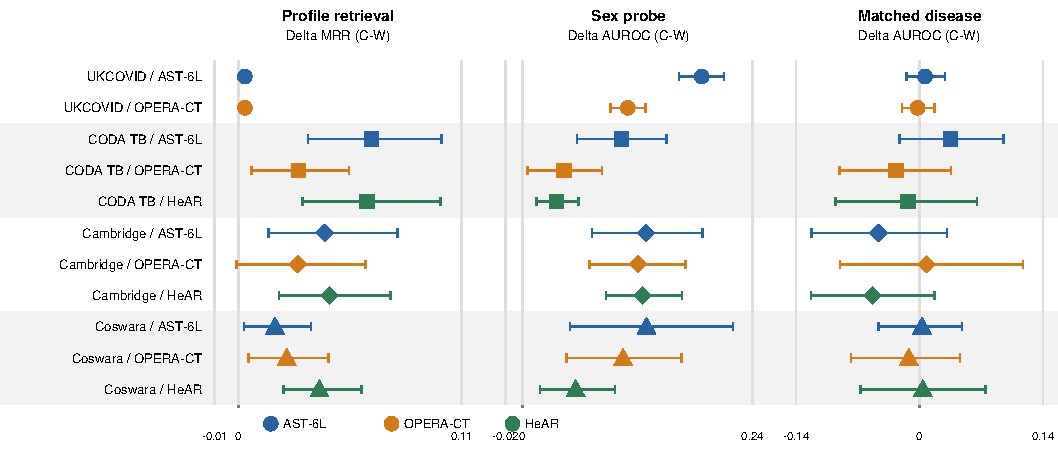
\includegraphics[width=0.98\textwidth]{cross_dataset_forest.pdf}
  \caption{Correct-minus-Within estimates with 95\% paired bootstrap intervals. The 11
  settings comprise UKCOVID (discovery: AST, OPERA) and three external sensitivities
  (AST, OPERA, HeAR each). Retrieval CIs excluded zero in 10/11 settings and sex-probe CIs
  in 11/11, whereas no matched disease CI established a positive gain. Panel scales differ;
  estimates are not pooled because profile libraries, diseases, and evidence status differ.}
  \label{fig:forest}
\end{figure*}

\subsection{Correspondence did not robustly improve disease transfer}

On UKCOVID matched, disease \cw{} \dauc{} was $+0.0062$ [-0.0144, 0.0279] for AST and
$-0.0020$ [-0.0191, 0.0168] for OPERA. For AST, raw, Correct, and Within AUROC were 0.538,
0.529, and 0.523; for OPERA they were 0.577, 0.555, and 0.557. A small AST fusion effect
did not replicate with OPERA, and Correct fusion did not outperform metadata plus raw
audio. A fixed MLP also failed to reveal a hidden effect: audio-only \cw{} was $+0.0050$
[-0.0154, 0.0270] for AST and $-0.0052$ [-0.0208, 0.0110] for OPERA.

Figure~\ref{fig:forest} summarizes the external result shape. Across all 11
dataset--backbone settings, retrieval point estimates were positive (10/11 intervals
excluded zero) and sex \cw{} was positive with 11/11 intervals excluding zero. In contrast,
matched disease \cw{} produced five positive and six negative point estimates, and 0/11
intervals established a positive gain. This count is descriptive, not a meta-analysis:
targets contain different diseases, MRR libraries differ, and external analyses have
different evidence status. Correct likewise showed no consistent advantage over frozen raw
audio.

\subsection{Label association, fusion, and calibration}

Within-label and Global also separated in the source cohort. For UKCOVID AST, source
\wg{} probe \dauc{} was $+0.0646$ for COVID, $+0.0758$ for cough, and $+0.0647$ for
recruitment source; all three intervals excluded zero. On matched participants, the COVID
increment fell to $+0.0126$ with an interval crossing zero, while cough remained positive
($+0.0803$). Thus, label-conditioned metadata association is itself learnable and would be
conflated with exact pairing by a Correct-versus-Global comparison alone.

Direct fusion did not provide a robust alternative positive result. On UKCOVID matched,
adding raw audio to metadata changed AUROC by only $+0.0028$ [-0.0016, 0.0073] for AST and
$+0.0041$ [-0.0006, 0.0087] for OPERA. Metadata plus Correct exceeded metadata plus Within
for AST ($+0.0156$ [0.0034, 0.0276]) but not OPERA ($+0.0021$ [-0.0068, 0.0107]); neither
backbone's Correct fusion beat metadata plus raw audio. This isolates a small,
backbone-specific ranking signal rather than a reproducible alignment advantage.

With source calibration, UKCOVID Correct had worse matched NLL than Within, although
AUROC differences were negligible. The change in negative NLL was $-0.0249$
[-0.0443, -0.0069] for AST and $-0.0176$ [-0.0335, -0.0010] for OPERA. Target calibration
reduced both gaps to approximately zero without changing AUROC. The source NLL penalty
therefore primarily reflects confidence unsupported after cohort shift, not demonstrated
destruction of disease ranking; recalibration repairs probability scale but creates no
transferable discrimination.

\section{Discussion}
\label{sec:discussion}

The audit separates two outcomes that conventional evaluation can conflate. Correct
audio--metadata alignment repeatedly improved retrieval of participant profiles, proving
that genuine correspondence was learned. Yet the most reproducible additional channel was
participant sex, while disease improvements were small, directionally inconsistent, and
not robust to raw-audio controls or readout changes. In plain terms, the model became better
at matching a recording to the kind of participant described by a metadata card, but not
reliably better at diagnosing disease after measured patient composition was balanced.

Within-label shuffling is essential to this conclusion. Correct versus Global alone would
mix exact profile correspondence with label-conditioned population association. Retrieval
then verifies the manipulation, probes describe the retained channels, and matched
evaluation asks the clinical transfer question. Future clinical audio--metadata studies
should minimally report these controls together with a frozen raw reference and calibration
under population shift.

This changes how positive alignment results should be interpreted. Low alignment loss or
high profile retrieval establishes that paired supervision was absorbed; it does not say
which part of a heterogeneous profile was used. A source-domain disease gain can then arise
from label-conditioned patient composition, particularly when recruitment and label are
coupled. Only a prespecified participant-disjoint target that balances measured patient
context asks whether the gain survives the intended population change. Pairing is therefore
a manipulation check, probes are representation diagnostics, and matched disease prediction
is the transfer endpoint.

The recurring sex result also requires careful wording. A probe shows that sex is decodable,
not that the disease classifier causally relies on it. Moreover, raw audio often contains
more demographic information than any aligned representation. Correct therefore appears to
preserve this channel relative to a Within-label projector rather than create a new
demographic attribute. This distinction prevents a large \cw{} probe effect from being
misread as participant identification or newly introduced bias.

The evidence remains bounded. UKCOVID is a discovery audit; CODA, Cambridge, and Coswara
are secondary or post-hoc sensitivities with 100-pair targets and wide intervals. Matching
balances measured covariates only, probes do not establish causal use, and the experiment
audits one Stage-1-style projector rather than a complete multimodal reasoning system.
Our synthetic study also failed its preregistered general-mechanism gates, so these recurring
patterns are not presented as a universal causal law. A proposed disease-invariant repair
was not trained because the available single-dataset cohorts lacked the prespecified support
for cross-environment same-label positives and within-environment opposite-label negatives.
This is a data-feasibility limitation, not a negative result for the repair method.

\section{Conclusion}

Correct pairing reproducibly improved participant-profile correspondence, especially sex,
but did not yield a robust cross-backbone improvement in covariate-balanced disease
prediction or consistently outperform raw audio. Successful audio--metadata correspondence
is therefore not sufficient evidence of a transferable disease representation;
correspondence, retained information, and disease transfer must be evaluated separately.

\section*{Compliance with Ethical Standards}
This work is a secondary analysis of de-identified datasets accessed and used under their
respective data-use terms. No new participants were recruited and no clinical decisions
were made from model outputs.

\bibliographystyle{IEEEbib}
\bibliography{references}

\end{document}
